% -*- TeX-engine: luatex -*-
\documentclass[presentation,aspectratio=43, 10pt]{beamer}
\usepackage{booktabs}
\titlegraphic{\hfill
\includegraphics[height=1.25cm]{durham-logo}}
\def\xunderbrace#1_#2{{\underbrace{#1}_{\mathclap{#2}}}}
\def\xoverbrace#1^#2{{\overbrace{#1}^{\mathclap{#2}}}}
\def\xunderarrow#1_#2{{\underset{\overset{\uparrow}{\mathclap{#2}}}{#1}}}
\def\xoverarrow#1^#2{{\overset{\underset{\downarrow}{\mathclap{#2}}}{#1}}}

\usepackage{appendixnumberbeamer}
\usepackage{amsmath}
\usepackage{amssymb}
\usepackage{mathtools}
\usepackage{hyperref}
\usepackage{xspace}
\newcommand{\arxivlink}[2]{{\texttt{arXiv:\,\href{https://arxiv.org/abs/#1}{#1\,[#2]}}}}

\newcommand{\eps}[1]{\ensuremath{\varepsilon{(#1)}}}
\newcommand{\honev}{\ensuremath{{H}^1(\Omega; \mathbb{R}^d)}\xspace}
\newcommand{\ltwov}{\ensuremath{{L}^2(\Omega; \mathbb{R}^d)}\xspace}
\newcommand{\ltwo}{\ensuremath{{L}^2(\Omega)}\xspace}
\newcommand{\inner}[1]{\left\langle #1 \right \rangle}
\newcommand{\dx}{\,\text{d}x}
\newcommand{\ds}{\,\text{d}s}

\date{2021-09-09}
\usepackage{minted}
\usepackage[url=false,
doi=true,
isbn=false,
style=authoryear,
maxnames=5,
giveninits=true,
uniquename=init,
backend=biber]{biblatex}
\renewcommand{\bibfont}{\fontsize{7}{7}\selectfont}
\addbibresource{references.bib}

\setlength{\bibitemsep}{1ex}
\setlength{\fboxsep}{1pt}

\renewbibmacro{in:}{}
\DeclareFieldFormat[article]{volume}{\textbf{#1}}
\DeclareFieldFormat{doi}{%
  doi\addcolon%
  {\scriptsize\ifhyperref{\href{http://dx.doi.org/#1}{\nolinkurl{#1}}}
    {\nolinkurl{#1}}}}
\AtEveryBibitem{%
\clearfield{pages}%
\clearfield{issue}%
\clearfield{number}%
}

\DeclareMathOperator{\grad}{grad}
\let\div\relax
\DeclareMathOperator{\div}{div}
\DeclareMathOperator{\curl}{curl}
\DeclareMathOperator{\range}{range}
\DeclareMathOperator{\sym}{sym}
\newcommand{\advect}[2]{\ensuremath{(#2 \cdot \nabla) #1}}
\newcommand{\kerdiv}{\ker\div}
\newcommand{\kercurl}{\ker\curl}
\let\Re\relax
\DeclareMathOperator{\Re}{Re}

\usetheme{metropolis}
\setbeamertemplate{title graphic}{
  \vbox to 0pt {
    \vspace*{1em}
    \inserttitlegraphic%
  }%
  \nointerlineskip%
}
\metroset{background=light,progressbar=frametitle,numbering=counter,block=fill}

% https://www.dur.ac.uk/marketingandcommunications/marketing/branding/colourpalette/
% Most of these are indistinguishable to those suffering colour blindness
\definecolor{purple}{HTML}{68246D}
\definecolor{blue}{HTML}{002A41}
\definecolor{red}{HTML}{BE1E2D}
\definecolor{cyan}{HTML}{00AEEF}
\definecolor{yellow}{HTML}{FFD53A}

\newenvironment{variableblock}[3]
{\setbeamercolor{block body}{#2}
\setbeamercolor{block title}{#3}
\begin{block}{#1}}%
{\end{block}}
  
\newenvironment{challenge}[1]%
{\begin{variableblock}{#1}{bg=red!20,fg=black}{bg=red,fg=white}}%
{\end{variableblock}}

\newenvironment{answer}[1]%
{\begin{variableblock}{#1}{bg=cyan!20,fg=black}{bg=cyan,fg=white}}%
{\end{variableblock}}

\renewenvironment{exampleblock}[1]%
{\begin{variableblock}{#1}{bg=yellow!20,fg=black}{bg=yellow,fg=white}}%
{\end{variableblock}}

\setbeamercolor{normal text}{
  fg=black,
  bg=white
}
\setbeamercolor{alerted text}{
  fg=red
}
\setbeamercolor{example text}{
  fg=blue
}

\setbeamercolor{palette primary}{%
  use=normal text,
  fg=normal text.bg,
  bg=purple,
}

\usetheme{metropolis}

\author{Lawrence Mitchell\inst{1,*}
\\ {\scriptsize with: Colin Cotter (Imperial) Patrick Farrell, Fabian
    Laakmann (Oxford), Matt Knepley (Buffalo), Florian Wechsung
    (NYU)}
}
\institute{
  \inst{1}Department of Computer Science, Durham University\\
  \inst{*}\texttt{lawrence.mitchell@durham.ac.uk}
}

\title{Augmented Lagrangian preconditioning for fluids: theory and practice}

\usepackage{tikz}
\usetikzlibrary{trees,calc,positioning}
\usetikzlibrary{shapes, shapes.geometric}
\usetikzlibrary{arrows,chains,positioning,fit,backgrounds,calc,shapes,
  shadows,scopes,decorations.markings,plotmarks}
\usepackage{tikz-cd}
\usepackage{standalone}
\newcommand*{\tettextsize}{\footnotesize}
\tikzstyle{line} = [draw, -, thick]
\tikzstyle{nodraw} = [draw, fill, circle, minimum width=0pt, inner sep=0pt]
\tikzstyle{sieve} = [line, circle, font=\tettextsize, inner sep=0pt,
  minimum size=12pt]

\usepackage{pgf}
\usepackage{pgfplots}
\usepackage{pgfplotstable}

\tikzstyle{cell} = [sieve, fill=blue!60]
\tikzstyle{facet} = [sieve, fill=green!35]
\tikzstyle{edge} = [sieve, fill=red!35]
\tikzstyle{vertex} = [sieve, fill=blue!35]

% https://tex.stackexchange.com/questions/27171/padded-boundary-of-convex-hull
\newcommand{\convexpath}[2]{
  [
  create hullcoords/.code={
    \global\edef\namelist{#1}
    \foreach [count=\counter] \nodename in \namelist {
      \global\edef\numberofnodes{\counter}
      \coordinate (hullcoord\counter) at (\nodename);
    }
    \coordinate (hullcoord0) at (hullcoord\numberofnodes);
    \pgfmathtruncatemacro\lastnumber{\numberofnodes+1}
    \coordinate (hullcoord\lastnumber) at (hullcoord1);
  },
  create hullcoords
  ]
  ($(hullcoord1)!#2!-90:(hullcoord0)$)
  \foreach [
  evaluate=\currentnode as \previousnode using \currentnode-1,
  evaluate=\currentnode as \nextnode using \currentnode+1
  ] \currentnode in {1,...,\numberofnodes} {
    let \p1 = ($(hullcoord\currentnode) - (hullcoord\previousnode)$),
    \n1 = {atan2(\y1,\x1) + 90},
    \p2 = ($(hullcoord\nextnode) - (hullcoord\currentnode)$),
    \n2 = {atan2(\y2,\x2) + 90},
    \n{delta} = {Mod(\n2-\n1,360) - 360}
    in
    {arc [start angle=\n1, delta angle=\n{delta}, radius=#2]}
    -- ($(hullcoord\nextnode)!#2!-90:(hullcoord\currentnode)$)
  }
}

\graphicspath{{./\jobname.figures/}{../pictures/}}

\usepackage{emoji}

\begin{document}
\maketitle

% \begin{abstract}
%   Augmented Lagrangian preconditioning for fluids problems was
%   introduced by Benzi and Olshanskii in 2006. The approach offers excellent,
%   parameter-robust, control of the Schur complement approximation. The
%   drawback is that the preconditioning scheme for the top-left block
%   is significantly more complicated, and at the time, an extension to
%   three dimensions was not known.

%   In recent years, there has been significant progress in this area,
%   guided by a deeper understanding of how to construct appropriate
%   preconditioners, and software advances that ease implementation.

%   The core idea in the design of effective preconditioners for the top
%   left block is characterising a basis for the kernel of the augmented
%   Lagrangian term. Structure preserving discretisations offer a
%   systematic way to attack this problem when the augmentation is a
%   differential operator. The resulting robust multigrid methods
%   require small block overlapping additive Schwarz smoothers.

%   In this talk I will discuss the general augmented Lagrangian
%   approach, discuss a flexible preconditioning package that provides
%   fast implementation of optimal methods, and illustrate with some
%   examples covering stationary Navier--Stokes and MHD, along with
%   time-dependent problems.
% \end{abstract}


\begin{frame}
  \frametitle{A first problem}
  \begin{block}{Stationary, Newtonian, incompressible Navier--Stokes}
    Find $(u, p) \in \honev \times \ltwo$ such that
    \begin{alignat*}{2}
      -  \nu \nabla^2 u + \advect{u}{u} + \nabla p &= f \quad && \text{ in } \Omega, \\
      \nabla \cdot u &= 0 \quad && \text{ in } \Omega,
    \end{alignat*}
    with suitable boundary conditions, and $\nu$ the kinematic viscosity.
  \end{block}
  \begin{exampleblock}{Multiple solutions}<2->
    For $\nu \to 0$, these equations admit multiple solutions
  \end{exampleblock}
  \begin{challenge}{Motivating question}<3->
    What are the solution(s) as $\nu$ varies?
  \end{challenge}
\end{frame}

\begin{frame}
  \frametitle{Challenges for solvers}
  \begin{challenge}{Desired properties}
    \begin{itemize}
    \item Growth in time to solution is (at worst)
      $\mathcal{O}(n\log n)$ in number of degrees of freedom (resolution).
    \item Convergence does not degrade with $\nu \to 0$.
    \end{itemize}
  \end{challenge}
  \begin{columns}[t]
    \begin{column}{0.48\textwidth}
      \begin{block}{Direct methods}
        \begin{itemize}
        \item[\emoji{thumbsup}] Convergence independent of $\nu$
        \item[\emoji{thumbsdown}] Time to solution $\mathcal{O}(n^2)$ (3D).
        \end{itemize}
      \end{block}
    \end{column}
    \begin{column}{0.48\textwidth}
      \begin{block}{Krylov methods}
        \begin{itemize}
        \item[\emoji{thumbsup}] Time to solution $\mathcal{O}(n \log n)$ (with
          multilevel preconditioner)
        \item[\emoji{thumbsdown}] Convergence independent of $\nu$ challenging
        \end{itemize}
      \end{block}
    \end{column}
  \end{columns}
\end{frame}

\begin{frame}
  \frametitle{Block preconditioning}
  \begin{exampleblock}{Newton linearisation}
    \begin{equation*}
      P := \begin{pmatrix}
        A & B^T \\
        B & 0
      \end{pmatrix}
      \begin{pmatrix}
        \delta u \\ \delta p
      \end{pmatrix}
      =
      \begin{pmatrix}
        b \\ 0
      \end{pmatrix}.
    \end{equation*}
  \end{exampleblock}
  \pause
  \begin{answer}{Block factorisations}
    \begin{equation*}
      P^{-1} =
      \begin{pmatrix}
        I   & -A^{-1} B^T \\
        0 & I \\
      \end{pmatrix}
      \begin{pmatrix}
        A^{-1}  & 0 \\
        0 & S^{-1} \\
      \end{pmatrix}
      \begin{pmatrix}
        I   & 0 \\
        -BA^{-1} & I \\
      \end{pmatrix}
    \end{equation*}
  \end{answer}
  \begin{challenge}{PDE-specific challenge}
    Find good approximations $\tilde{A}^{-1}$ for $A^{-1}$ and
    $\tilde{S}^{-1}$ for $S^{-1}$.
  \end{challenge}
\end{frame}

\begin{frame}
  \frametitle{What about that Schur complement?}
  \begin{columns}
    \begin{column}{0.55\textwidth}
      Want an approximation $\tilde{S}^{-1}$ that
      \begin{enumerate}
      \item is robust to parameter variation
      \item is cheap to construct/apply
      \item scales well in parallel
      \end{enumerate}

      Generally (1) is the hardest to satisfy.

      $\Rightarrow$ augmented Lagrangian approach.
    \end{column}
    \begin{column}{0.45\textwidth}
      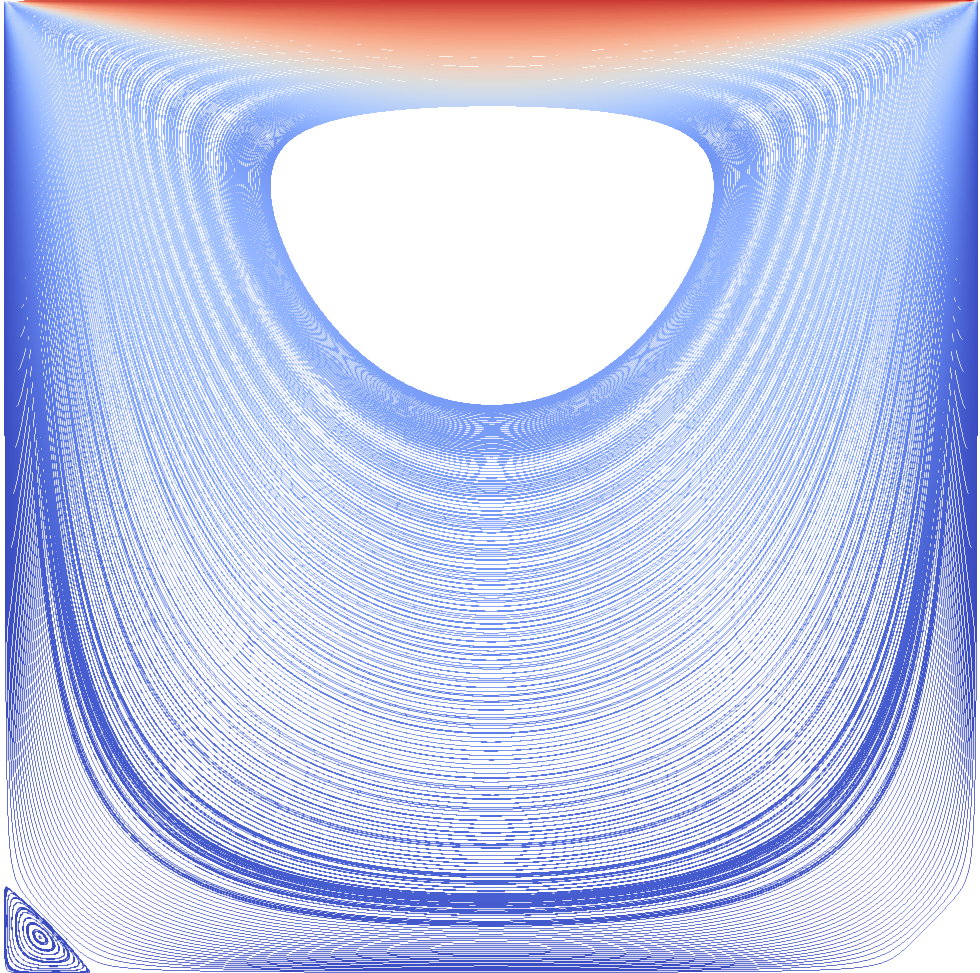
\includegraphics[width=0.333\textwidth]{mhd/ldc_1_1_u}%
      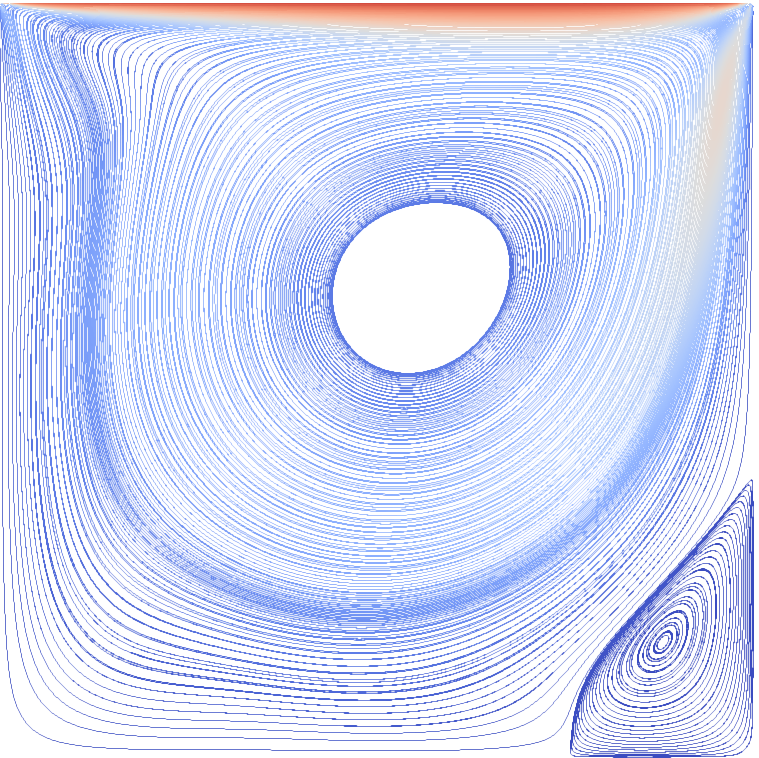
\includegraphics[width=0.333\textwidth]{mhd/ldc_500_500_u}%
      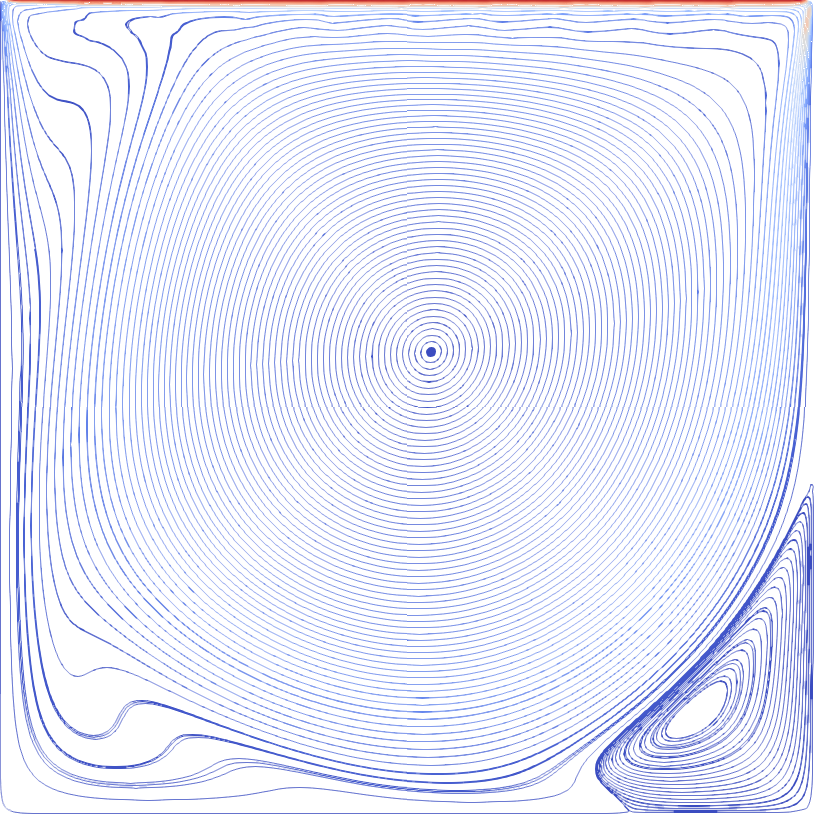
\includegraphics[width=0.333\textwidth]{mhd/ldc_5000_5000_u}%
      \\
      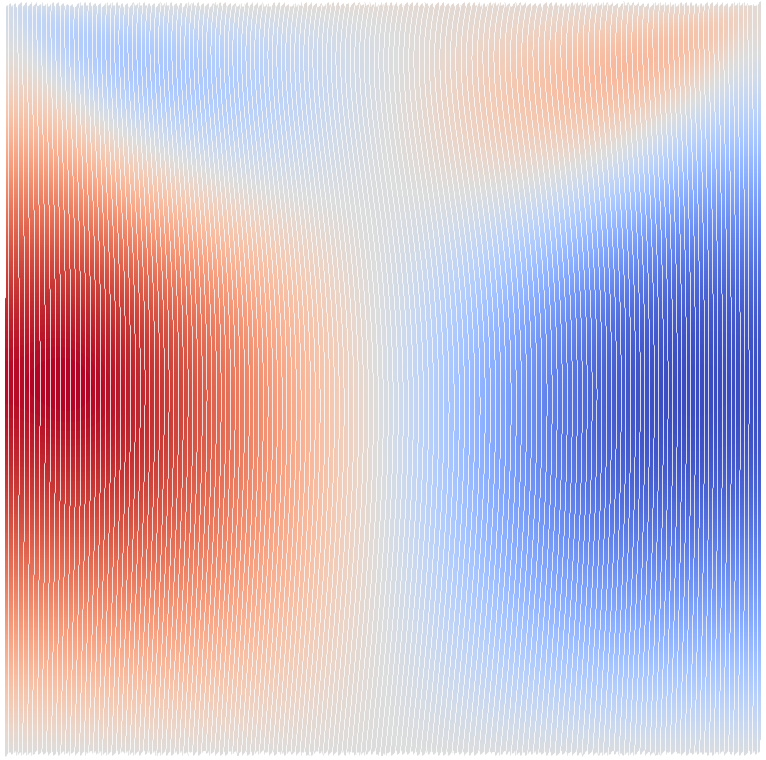
\includegraphics[width=0.333\textwidth]{mhd/ldc_1_1_B}%
      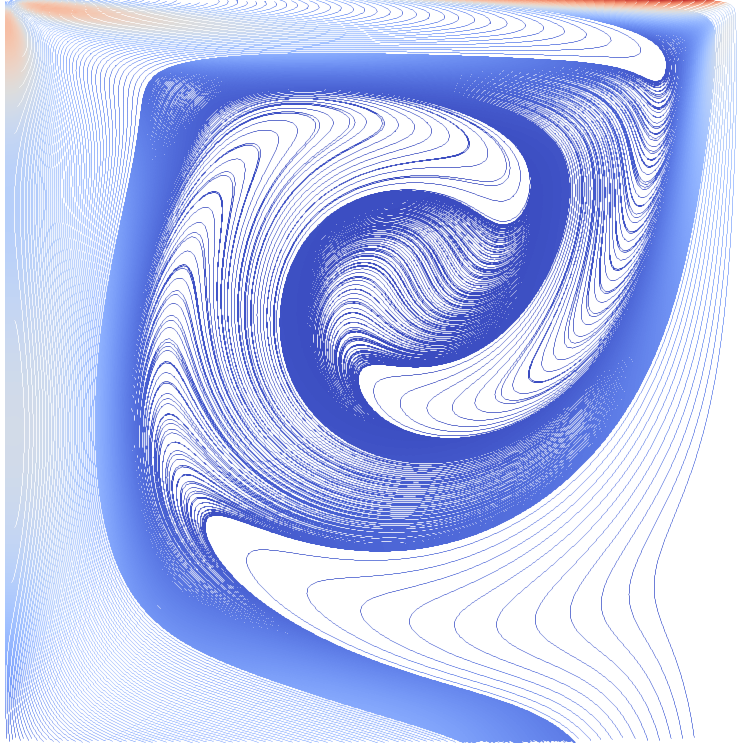
\includegraphics[width=0.333\textwidth]{mhd/ldc_500_500_B}%
      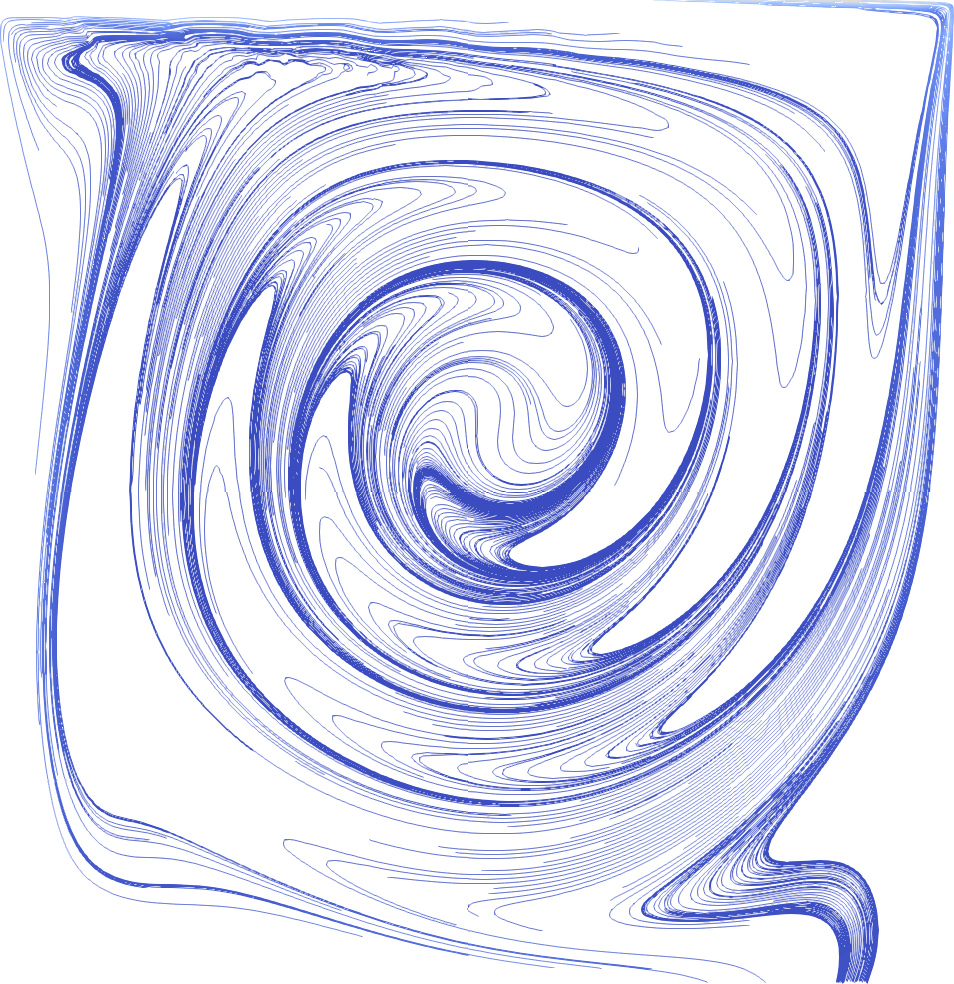
\includegraphics[width=0.333\textwidth]{mhd/ldc_5000_5000_B}%

      \vspace{2em}
      {\raggedleft\scriptsize
        \textcite{Laakmann:2021} \arxivlink{2104.14855}{math.NA}\par}
    \end{column}
  \end{columns}
\end{frame}

\begin{frame}
  \frametitle{Controlling the Schur complement: augmented
    Lagrangian}
  \begin{exampleblock}{Continuous augmentation}
    Add $\gamma \grad\div u$ term to the momentum equation.

    Doesn't change solution since $\div u = 0$
  \end{exampleblock}
  \begin{theorem}[Hestenes, Fortin, Glowinski, Olshanksii, \dots]
    As $\gamma \to \infty$, the Schur complement is well
    approximated by $\tilde{S}^{-1} = -(\nu + \gamma)M_p^{-1}$.
  \end{theorem}
  \pause
  \begin{exampleblock}{Discrete augmentation}
    \begin{equation*}
      \begin{pmatrix}
        A + \gamma B^T M_p^{-1} B & B^T \\
        B & 0
      \end{pmatrix}
      \begin{pmatrix}
        u \\ p
      \end{pmatrix}
      =
      \begin{pmatrix}
        b \\ 0
      \end{pmatrix}
    \end{equation*}

    Doesn't change solution since $B u = 0$.

    Again, as $\gamma \to \infty$, $S^{-1}$ is well approximated by
    $\tilde{S}^{-1} = -(\nu + \gamma)M_p^{-1}$.
  \end{exampleblock}
\end{frame}
\begin{frame}
  \frametitle{Why does this work?}
  \begin{answer}{New Schur complement}
    \begin{equation*}
    \begin{aligned}
      S^{-1} &= -(B(A+\gamma B^T M_p^{-1} B)^{-1} B^T)^{-1} \\
      &= -(B(A^{-1} - \gamma A^{-1} B^T(M_p + B A^{-1} B^T)^{-1}BA^{-1})B^T)^{-1}\\
      &= -(\underbrace{BA^{-1}B^T}_{\Lambda} - \gamma BA^{-1}B^T (M_p + BA^{-1} B^T)^{-1}BA^{-1}B^T)^{-1}\\
      &= -(\Lambda^{-1} + \gamma \Lambda^{-1}\Lambda(M_p + \Lambda - \Lambda \Lambda^{-1}\Lambda)^{-1}\Lambda \Lambda^{-1}) \\
      &= -(BA^{-1}B^T)^{-1} - \gamma M_p^{-1}.\\
    \end{aligned}
  \end{equation*}
   approximate commutator argument (ignoring advection):
   \begin{equation*}
     BA^{-1}B^T \approx \nu BB^TA^{-1} \approx \nu M_p^{-1}
   \end{equation*}
  \end{answer}
\end{frame}

\begin{frame}
  \frametitle{Conservation of misery}
  \begin{exampleblock}{Good news}
    \emoji{thumbsup} The Schur complement becomes easy to approximate as $\gamma \to \infty$
  \end{exampleblock}
  \begin{challenge}{Bad news}
    \emoji{thumbsdown} The scalable solver we had for $\tilde{A}^{-1}$ doesn't work for
    $A_\gamma := A + \gamma B^T M_p^{-1} B$
  \end{challenge}
  \pause
  \begin{center}
    \begin{tabular}{l| c |c}
      \toprule
      &  LU for $\tilde{A}_\gamma^{-1}$ & AMG for $\tilde{A}_\gamma^{-1}$\\
      \midrule
      $\gamma=10^{-1}$ & 15 &18\\
      $\gamma=1$ & 6 &40\\
      $\gamma=10^{1}$ & 3 &107\\
      \bottomrule
    \end{tabular}

    Outer Krylov iterations for different choices of $\tilde{A}^{-1}_\gamma$.
  \end{center}
\end{frame}

\begin{frame}
  \frametitle{$\gamma$-robust multigrid I}
  \begin{itemize}
  \item Ignorning advection, then the top-left block corresponds to
    discretisation of
    \begin{equation*}
      a_{\gamma}(u, v) = \xunderbrace{\int_\Omega 2\nu \eps{u}  :
        \eps{v} \dx}_{\text{sym.~pos.~def.}} \quad +  \quad
      \textcolor{red}{\xunderbrace{\int_\Omega \gamma\div u\div v \dx}_{\text{sym.~pos.~semi-def.}}}
    \end{equation*}
    \pause
  \item The semi-definite term is singular on all solenoidal fields
    $\Rightarrow$ the system becomes \emph{nearly singular} as $\gamma
    \to \infty$
    \pause
  \item To build a $\gamma$-robust scheme we need
    \parencite{Schoeberl:1999}
    \begin{itemize}
    \item a $\gamma$-robust smoother;
    \item a prolongation operator with $\gamma$-independent continuity
      constant;
    \item[$\Rightarrow$] overlapping Schwarz smoother with
      decomposition that decomposes the kernel. ``The right blocks for
      block Jacobi''.
    \item First application to NS: $P_2$-$P_0$ (2D) \parencite{Benzi:2006}
    \end{itemize}
  \end{itemize}
\end{frame}

\begin{frame}
  \frametitle{$\gamma$-robust multigrid II}
  Consider the problem: for
  $\gamma \in \mathbb{R}_+$, find $u \in V$ such that
  \begin{equation*}
    a(u, v) + \gamma b(u, v) = (f, v) \quad \forall v \in V,
  \end{equation*}
  where $a$ is SPD, and $b$ is symmetric positive semidefinite.

  This matches our problem (ignoring advection) with $a = \nu (\eps{u},
  \eps{v})$ and $b = (\div u, \div v)$.
  \pause
  \begin{theorem}[Sch\"oberl (1999); Lee, Wu, Xu, Zikatanov (2007)]
    {\small
    Let the kernel be
    \begin{equation*}
      \mathcal{N} := \{ u \in V : b(u, v) = 0 \,\, \forall v \in V \}.
    \end{equation*}
    A Schwarz smoother whose decomposition $V = \sum_i
    V_i$ satisfies
    \begin{equation*}
      \mathcal{N} = \sum_i \mathcal{N} \cap V_i,
    \end{equation*}
    is robust wrt $\gamma$.
    \nocite{Schoeberl:1999,Lee:2007}
    }
  \end{theorem}
\end{frame}

\begin{frame}[fragile]
  \frametitle{Toolkit for construction of $V_i$: discrete Hilbert complexes}
  \begin{exampleblock}{Stokes complex}
    In 2D, the Stokes complex and S--V subcomplex are
    \begin{center}
      \begin{tikzcd}
        H^2 \arrow[r, "\curl"] \arrow[d] & \mathbf{H}^1 \arrow[r,
        "\div"]
        \arrow[d] & L^2 \arrow[d] \\
        \mathbb{HCT}_{k+1} \arrow[r, "\curl"] & (\mathbb{CG}_k)^2
        \arrow[r, "\div"] & \mathbb{DG}_{k-1}
      \end{tikzcd}
      \includestandalone[width=0.52\textwidth]{../pictures/HCT-complex}
    \end{center}
    Analogous complex in 3D (no pictures) due to \textcite{Fu:2018}.
    \begin{center}
      \begin{tikzcd}
        H^2 \arrow[r, "\grad"] & \mathbf{H}^1(\curl) \arrow[r,
        "\curl"] & \mathbf{H}^1 \arrow[r, "\div"] & L^2
      \end{tikzcd}
    \end{center}
  \end{exampleblock}
\end{frame}

\begin{frame}
  \frametitle{A picture}
  \begin{answer}{Idea}
    \begin{enumerate}
    \item Pick velocity space
    \item Walk left along complex
    \item Pick $V_i$ to cover support of the $\mathbb{HCT}$ basis.
    \end{enumerate}
  \end{answer}
    Giving a \emph{macrostar} decomposition around each vertex in the mesh.
    \begin{center}
      \includestandalone[height=0.3\textheight]{../pictures/macro-star}
    \end{center}
\end{frame}

\begin{frame}
  \frametitle{Numerical results --- 2D lid-driven cavity}
  \begin{table}[htbp]
    \centering
    \begin{tabular}{cc|ccccc}
      \toprule
      \# ref. & \# dofs & \multicolumn{5}{c}{Reynolds number} \\
              && 10 & 100 & 1000 & 5000 & 10000 \\
      \midrule
      1 & $9.3 \times 10^4$ & 2.50 & 2.33 & 2.33 & 5.50 & 8.50 \\
      2 & $3.7 \times 10^5$ & 2.00 & 2.00 & 2.00 & 4.00 & 6.00 \\
      3 & $1.5 \times 10^6$ & 2.00 & 1.67 & 1.67 & 2.50 & 3.50 \\
      4 & $5.9 \times 10^6$ & 2.00 & 1.67 & 1.50 & 1.50 & 4.00 \\
      \bottomrule
    \end{tabular}
    \caption{Average number of outer Krylov iterations per Newton step
      for a 2D regularised lid-driven cavity problem with
      $(\mathbb{CG}_3)^{2}-\mathbb{DG}_2$ pair.}
  \end{table}
  \begin{flushright}
    {\scriptsize
    P.E.~Farrell, \textbf{L.~Mitchell}, L.R.~Scott, and F.~Wechsung,
    SMAI JCM (2021).
    \arxivlink{2004.09398}{math.NA}\nocite{Farrell:2021a}
    }
  \end{flushright}
\end{frame}

\begin{frame}
  \frametitle{Numerical results --- 3D lid-driven cavity}
  \begin{table}[htbp]
    \centering
    \begin{tabular}{cc|ccccc}
      \toprule
      \# ref. & \# dofs & \multicolumn{5}{c}{Reynolds number} \\
              && 10 & 100 & 1\,000 & 2\,500 & 5\,000 \\
      \midrule
      1   & $1.03\times 10^6$     & 3.00  & 3.67  & 3.50 & 4.00 & 5.00\\
      2   & $8.22\times 10^6$     & 3.50  & 3.67  & 4.00 & 4.00 & 4.00\\
      3   & $6.55\times 10^7$     & 3.00  & 3.33  & 3.50 & 3.50 & 4.00\\
      \bottomrule
    \end{tabular}
    \caption{Average number of outer Krylov iterations per Newton step for a
      3D regularised lid-driven cavity problem with
      $(\mathbb{CG}_3)^{2}-\mathbb{DG}_2$ pair.}
  \end{table}
  \begin{flushright}
    {\scriptsize
    P.E.~Farrell, \textbf{L.~Mitchell}, L.R.~Scott, and F.~Wechsung,
    SMAI JCM (2021).
    \arxivlink{2004.09398}{math.NA}\nocite{Farrell:2021a}
    }
  \end{flushright}
\end{frame}

\begin{frame}[t]
  \frametitle{Computational performance --- 3D}
  % [53.140734383333324, 68.56801668333334, 61.468243016666655, 65.64923281666665]
  \pgfplotstableread[col sep=comma, row sep=\\]{%
    Cores,Time,Dofs\\
    48,5.3e1,2134839\\
    384,6.9e1,16936779\\
    3072,6.1e1,134930451\\
    24576,6.6e1,1077196323\\
  }\ldctable
  % [55.02509561666667, 68.57286605, 57.029964033333336, 69.39903468333333]
  \pgfplotstableread[col sep=comma, row sep=\\]{%
    Cores,Time,Dofs\\
    48,5.5e1,2107839\\
    384,6.9e1,16534263\\
    3072,5.7e1,130973115\\
    24576,6.9e1,1042606515\\
  }\bfstable
  \begin{columns}
    \begin{column}{0.5\textwidth}
      \begin{center}
        \begin{tikzpicture}
          \begin{semilogxaxis}[
            width=0.955\linewidth,
            height=0.9\linewidth,
            log basis x=2,
            ymin=0,
            ymax=80,
            xtick=data,
            xticklabels from table={\ldctable}{Cores},
            extra x ticks={48, 384, 3072, 24576},
            extra x tick labels={$[2.13]$, $[16.9]$,$[135]$,$[1077]$},
            extra x tick style={tick label style={yshift=-2.5ex}},
            xlabel={Cores\\{}[DoFs $\times 10^6$]},
            xlabel style={align=center, style={yshift=-0.5ex}},
            ylabel near ticks,
            ylabel style={align=center, text width=4cm},
            title={3D lid-driven cavity.},
            ylabel={Time [min]},
            ]
            \addplot+ table[x=Cores,y=Time] {\ldctable};
          \end{semilogxaxis}
        \end{tikzpicture}
      \end{center}
    \end{column}
    \begin{column}{0.5\textwidth}
      {\centering
        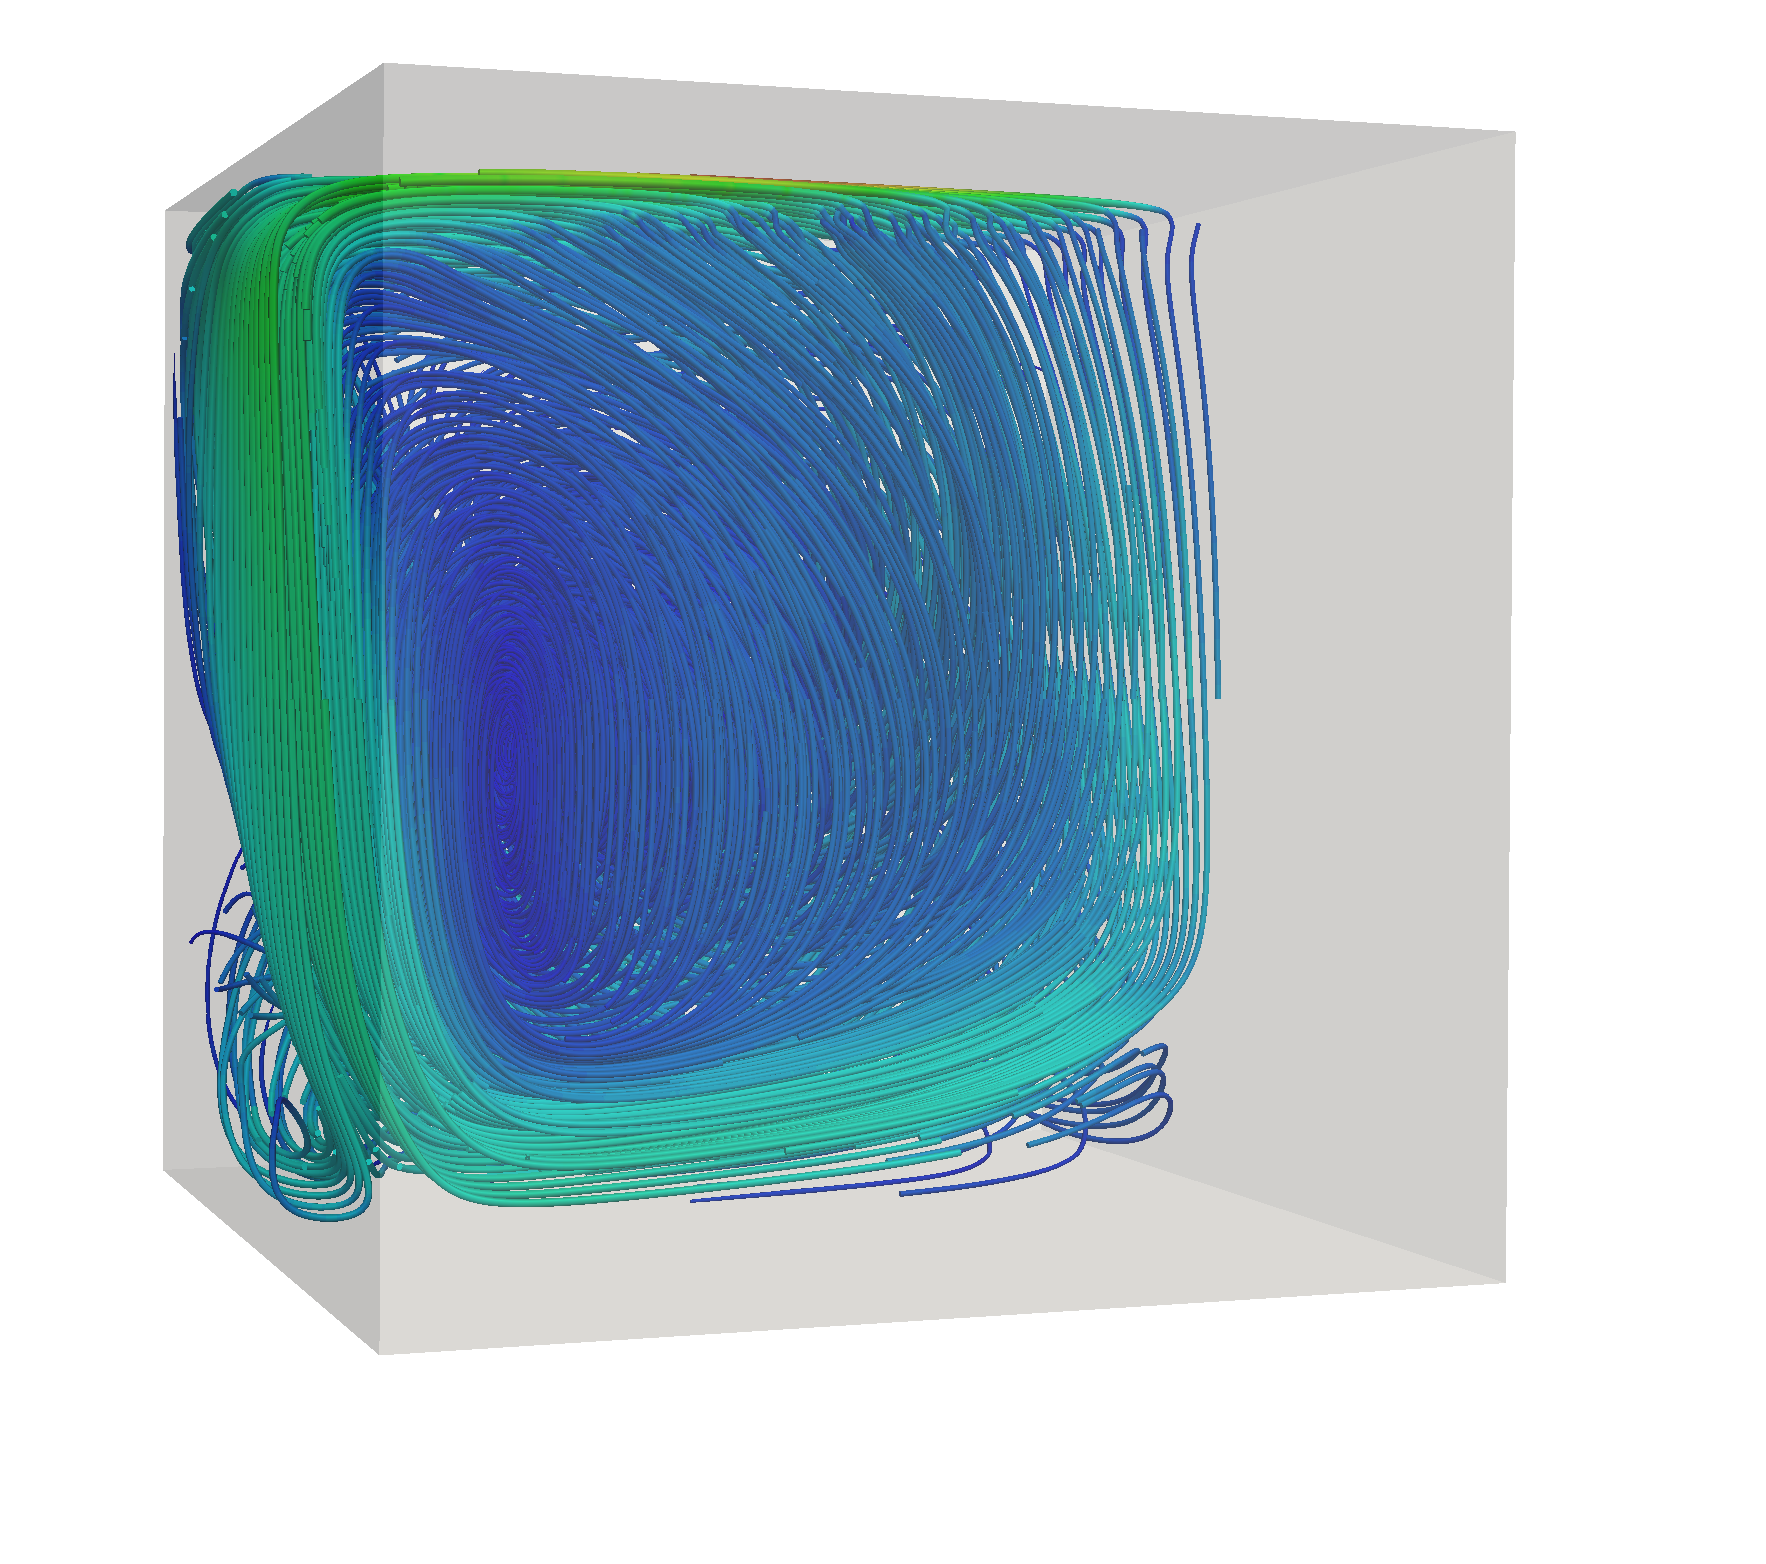
\includegraphics[width=\textwidth]{LDC-streamlines}}
      {\scriptsize Velocity streamlines at Reynolds number 5000.
        Credit F.~Wechsung, NYU.}
    \end{column}
  \end{columns}
  \begin{center}
    50 continuation steps
  \end{center}
\end{frame}

\begin{frame}
  \frametitle{AL for implicit timestepping}

  \begin{block}{Shallow water with compatible FEM}
    \begin{align*}
      u^{n+1} - u^{n} + \Delta t (u^{n+1/2} \cdot \nabla) u^{n+1/2} +
      \Delta t g h^{n+1/2} \\
      \alert{-\gamma \nabla\left(h^{n+1} - h^n + \Delta t \nabla
      \cdot (h^{n+1/2} u^{n+1/2})\right)} &= 0\\
      h^{n+1} - h^n + \Delta t \nabla \cdot (h^{n+1/2} u^{n+1/2}) &= 0
    \end{align*}
    After discretisation and linearisation, Schur complement
    approximation

    \begin{equation*}
      \tilde{S} \approx \gamma^{-1} L^{-1}(I - g \Delta t/2 L),
    \end{equation*}
    $L$ the Laplacian (or just ignore as $\Delta t \to \infty$).
  \end{block}
\end{frame}
\begin{frame}
  \frametitle{Preliminary results}
  {\scriptsize
    \centering
    \begin{tikzpicture}[%
      every node/.style={draw=black, thick, anchor=west},
      grow via three points={one child at (0.0,-0.7) and
        two children at (0.0,-0.7) and (0.0,-1.4)},
      edge from parent path={(\tikzparentnode.210) |- (\tikzchildnode.west)}]
      \node {Newton solver with line search}
      child { node {Krylov solver (FGMRES)}
        child { node {Block preconditioner}
          child { node {Approximate Schur complement inverse}
            child { node {$\tilde{S}^{-1} = M_\text{DG}^{-1}$ } }
          }
          child [missing] {}
          child { node {Geometric MG}
            child { node {Coarse grid solver}
              child { node {LU factorisation}}
            }
            child [missing] {}
            child { node {Relaxation}
              child { node {GMRES (3 iterations)}
                child { node {ASM smoother}}
              }
            }
          }
        }
      };
    \end{tikzpicture}
    \par}
\end{frame}
\begin{frame}
  \frametitle{Williamson mountain testcase}
  \begin{table}[htbp]
    \centering
    \begin{tabular}{cc|ccccc}
      \toprule
      \# ref. & \# cells & \# $h$ dofs & \# $u$ dofs & FGMRES its\\
      \midrule
      3   & 1280 & 3840 & 9600 & 6--7\\
      4 & 5120  & 15360 & 38400 & 6--7\\
      5 & 20480 & 61440 & 153600 & 6--7\\
      6 & 81920 & 245760 & 614400 & 6--7\\
      7 & 327680 & 983040 & 2457600 & 6--7\\
      \bottomrule
    \end{tabular}
    \caption{Krylov iterations per Newton step with
      $\Delta t = 1\text{hour}$}
  \end{table}

  {\centering
    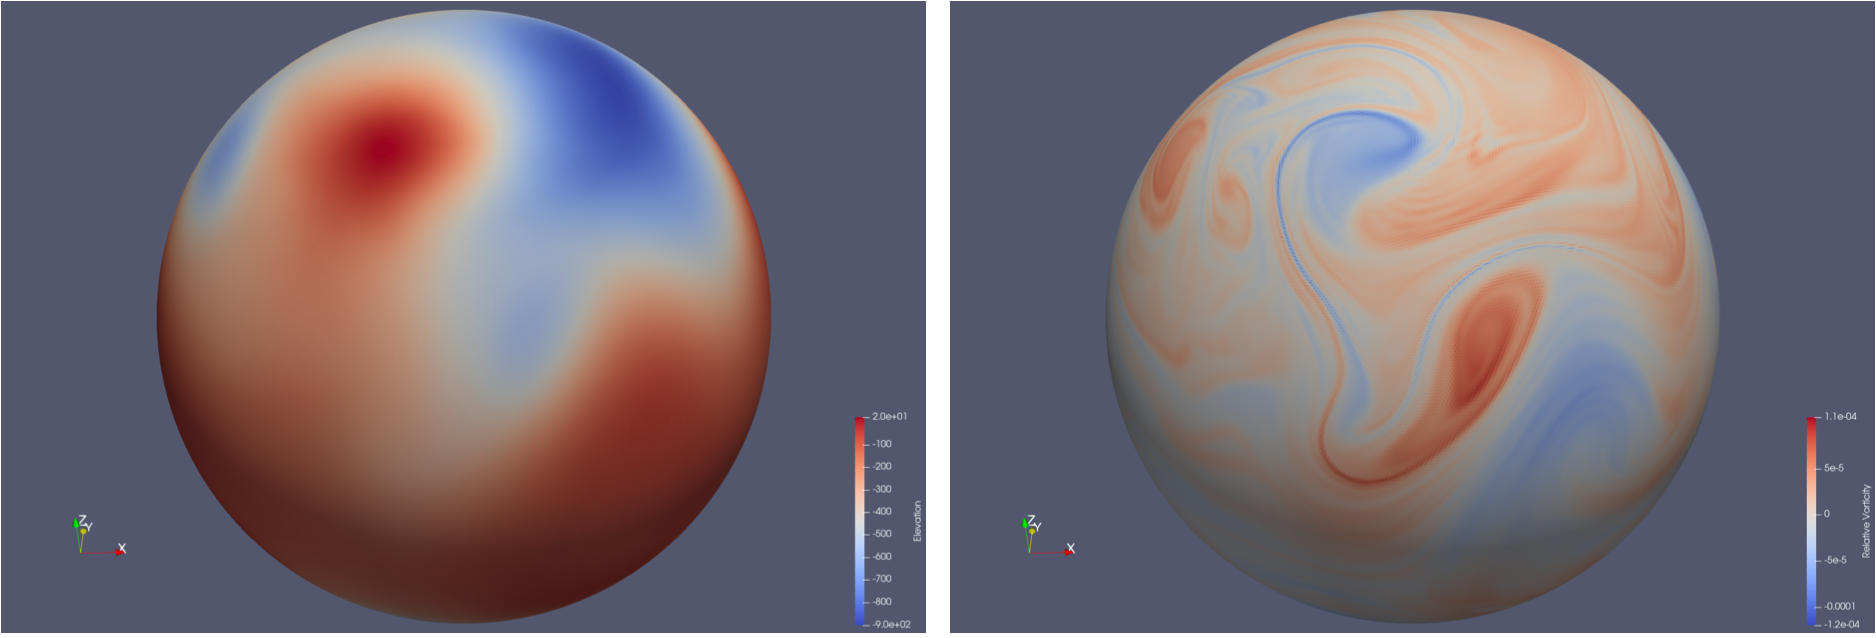
\includegraphics[height=0.4\textheight]{williamson-mountain-al}\par
    }
\end{frame}

\begin{frame}
  \frametitle{Computational technology: \texttt{PCPATCH} + Firedrake}
  General framework for small block overlapping Schwarz smoothers in
  PETSc and Firedrake

  \begin{itemize}
  \item Separate topological decomposition from algebraic operators
  \item Ask discretisation library to make the operators once
    decomposition is obtained
  \end{itemize}
  \begin{block}{Operators}
    \begin{columns}
      \begin{column}{0.65\textwidth}
        Callback interface to discretisation/PDE library.

        In this case, \url{www.firedrakeproject.org}
      \end{column}
      \begin{column}{0.2\textwidth}
        
\includegraphics[width=\textwidth]{firedrake}
      \end{column}
    \end{columns}
  \end{block}

  {\raggedleft
    \scriptsize \textcite{Farrell:2021b}, TOMS, \arxivlink{1912.08516}{cs.MS}\par}
\end{frame}

\begin{frame}
  \frametitle{Summary}
  \begin{itemize}
  \item AL formulation gives systematic way of producing Schur
    complement approximations for many problems
  \item Moves difficulty to development of appropriate additive
    Schwarz smoothers in multigrid
  \item[$\Rightarrow$] Discrete Hilbert complexes can guide this.
  \end{itemize}

  \begin{challenge}{Open questions}
    Really no theory for handling non-symmetric terms (mostly just
    ``hope GMRES helps enough'')

    Not super-efficient at high order

    Bigger block systems become expensive: all at once multigrid?
  \end{challenge}
\end{frame}
\appendix
\begin{frame}
  \frametitle{References}
  \printbibliography[heading=none]
\end{frame}

\end{document}
